\documentclass[11pt]{article}

\usepackage[utf8]{inputenc}
\usepackage[margin=1in]{geometry}
\usepackage{amsmath,amsthm,amssymb,graphicx,multicol,array,enumerate,textcomp}
\usepackage{tikz}
\usetikzlibrary{arrows.meta,calc}

\newenvironment{problem}[2][Problem]{\begin{trivlist}
\item[\hskip \labelsep {\bfseries #1}\hskip \labelsep {\bfseries #2.}]
\leavevmode\par
}{\end{trivlist}}

\newcommand{\usd}{\text{\$}}
\newcommand{\euro}{\text{\texteuro}}

\begin{document}

\title{Problem Set 8}
\author{Joe White\\ECO 442}
\maketitle

%--------------------------------------------------
\begin{problem}{1}

Suppose there is a decrease in the U.S. money supply.

\begin{enumerate}[(i)]

\item In the asset model, a decrease in the U.S. money supply shifts the real money supply curve left:
\[
\frac{MS_{\$}}{P_{\$}} \downarrow
\quad \Rightarrow \quad
R_{\$} \uparrow.
\]
The higher U.S. interest rate raises the return on dollar deposits in the foreign exchange market, so the dollar appreciates:
\[
E_{\$/\euro}\downarrow.
\]

\begin{center}
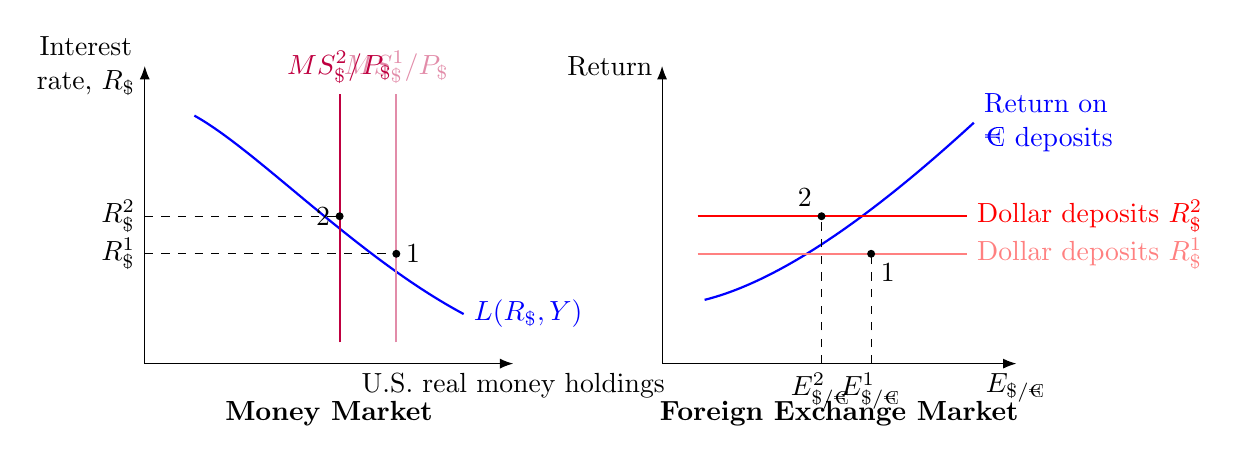
\begin{tikzpicture}[scale=0.9,>=Latex]

% ---------------- Money market ----------------
\begin{scope}[xshift=0cm]
\draw[->] (0,0) -- (0,4.2) node[left,align=center]{Interest\\rate, $R_{\$}$};
\draw[->] (0,0) -- (5.2,0) node[below]{U.S. real money holdings};

\draw[thick,blue] (0.7,3.5) .. controls (1.6,3.0) and (3.0,1.5) .. (4.5,0.7)
node[right] {$L(R_{\$},Y)$};

\draw[thick,purple!45] (3.55,0.3) -- (3.55,3.8) node[above] {$MS^1_{\$}/P_{\$}$};
\draw[thick,purple] (2.75,0.3) -- (2.75,3.8) node[above] {$MS^2_{\$}/P_{\$}$};

\fill (3.55,1.55) circle (1.6pt) node[right] {$1$};
\fill (2.75,2.08) circle (1.6pt) node[left] {$2$};

\draw[dashed] (0,1.55) -- (3.55,1.55);
\draw[dashed] (0,2.08) -- (2.75,2.08);

\node[left] at (0,1.55) {$R^1_{\$}$};
\node[left] at (0,2.08) {$R^2_{\$}$};

\node at (2.6,-0.7) {\textbf{Money Market}};
\end{scope}

% ---------------- FX market ----------------
\begin{scope}[xshift=7.3cm]
\draw[->] (0,0) -- (0,4.2) node[left]{Return};
\draw[->] (0,0) -- (5.0,0) node[below] {$E_{\$/\euro}$};

\draw[thick,blue] (0.6,0.9) .. controls (1.8,1.2) and (3.2,2.3) .. (4.4,3.4)
node[right,align=left] {Return on\\\euro\ deposits};

\draw[thick,red!50] (0.5,1.55) -- (4.3,1.55) node[right] {Dollar deposits $R^1_{\$}$};
\draw[thick,red] (0.5,2.08) -- (4.3,2.08) node[right] {Dollar deposits $R^2_{\$}$};

\fill (2.95,1.55) circle (1.6pt) node[below right] {$1$};
\fill (2.25,2.08) circle (1.6pt) node[above left] {$2$};

\draw[dashed] (2.95,0) -- (2.95,1.55);
\draw[dashed] (2.25,0) -- (2.25,2.08);

\node[below] at (2.95,0) {$E^1_{\$/\euro}$};
\node[below] at (2.25,0) {$E^2_{\$/\euro}$};

\node at (2.5,-0.7) {\textbf{Foreign Exchange Market}};
\end{scope}

\end{tikzpicture}
\end{center}

So the asset model prediction is:
\[
MS_{\$}\downarrow \Rightarrow R_{\$}\uparrow \Rightarrow E_{\$/\euro}\downarrow,
\]
meaning the dollar appreciates.

\item The AA schedule shifts down.  

At any given level of U.S. output, the fall in money supply raises U.S. interest rates, which increases the return on dollar deposits and causes the dollar to appreciate. Since the AA curve shows combinations of $Y$ and $E$ consistent with asset-market equilibrium, an exogenous appreciation shifts AA downward.

\item In the AA-DD model, DD does not shift because this is an asset-market shock, not a goods-market shock. AA shifts down, so short-run equilibrium moves to lower output and a lower exchange rate.

\begin{center}
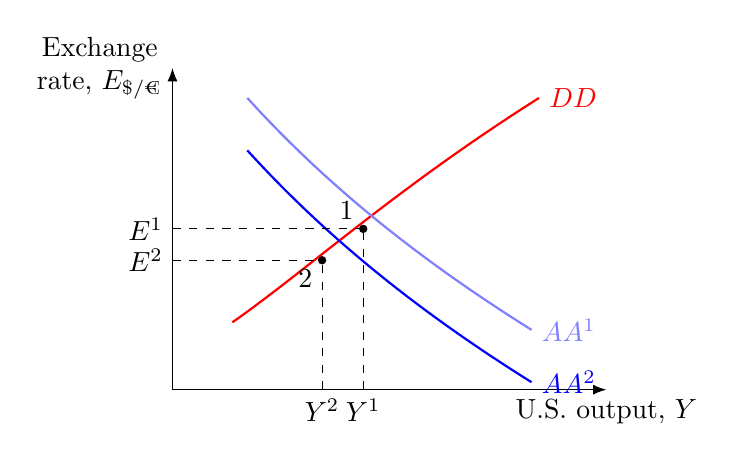
\begin{tikzpicture}[scale=0.95,>=Latex]
\draw[->] (0,0) -- (0,4.3) node[left,align=center]{Exchange\\rate, $E_{\$/\euro}$};
\draw[->] (0,0) -- (5.8,0) node[below]{U.S. output, $Y$};

\draw[thick,red] (0.8,0.9) .. controls (1.8,1.6) and (3.0,2.7) .. (4.9,3.9)
node[right] {$DD$};

\draw[thick,blue!50] (1.0,3.9) .. controls (2.0,2.8) and (3.2,1.8) .. (4.8,0.8)
node[right] {$AA^1$};

\draw[thick,blue] (1.0,3.2) .. controls (2.0,2.1) and (3.2,1.1) .. (4.8,0.1)
node[right] {$AA^2$};

\fill (2.55,2.15) circle (1.6pt) node[above left] {$1$};
\fill (2.00,1.73) circle (1.6pt) node[below left] {$2$};

\draw[dashed] (2.55,0) -- (2.55,2.15);
\draw[dashed] (0,2.15) -- (2.55,2.15);
\draw[dashed] (2.00,0) -- (2.00,1.73);
\draw[dashed] (0,1.73) -- (2.00,1.73);

\node[left] at (0,2.15) {$E^1$};
\node[left] at (0,1.73) {$E^2$};

\node[below] at (2.55,0) {$Y^1$};
\node[below] at (2.00,0) {$Y^2$};
\end{tikzpicture}
\end{center}

Therefore, in the short run:
\[
Y \downarrow,
\qquad
E_{\$/\euro}\downarrow.
\]
So U.S. real income falls, and the dollar appreciates.

\end{enumerate}

\end{problem}

%--------------------------------------------------
\begin{problem}{2}

\begin{enumerate}[(a)]

%-------------------- a --------------------
\item \textbf{An exogenous increase in investment spending by Japanese firms}

An increase in investment raises aggregate demand directly:
\[
D = C(Y-T)+I+G+CA\left(\frac{EP^*}{P},Y-T\right),
\]
so if $I\uparrow$, then $D\uparrow$. Therefore, the DD curve shifts right.  
The AA curve does not shift.

\begin{center}
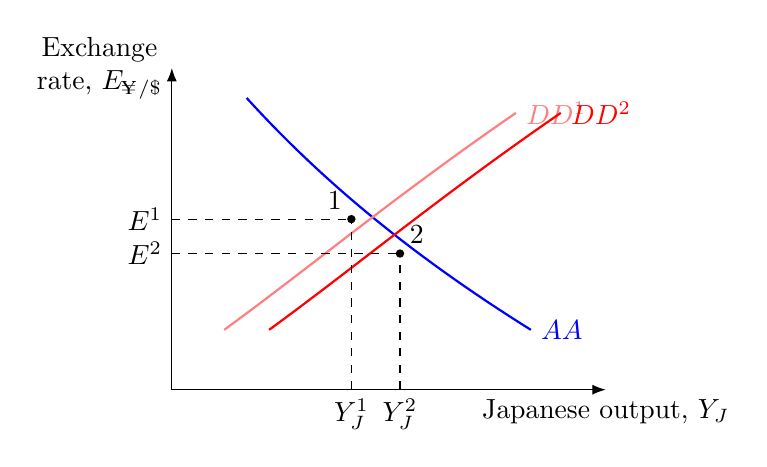
\begin{tikzpicture}[scale=0.95,>=Latex]
\draw[->] (0,0) -- (0,4.3) node[left,align=center]{Exchange\\rate, $E_{\text{¥}/\$}$};
\draw[->] (0,0) -- (5.8,0) node[below]{Japanese output, $Y_J$};

\draw[thick,blue] (1.0,3.9) .. controls (2.0,2.8) and (3.2,1.8) .. (4.8,0.8)
node[right] {$AA$};

\draw[thick,red!50] (0.7,0.8) .. controls (1.8,1.6) and (3.0,2.6) .. (4.6,3.7)
node[right] {$DD^1$};

\draw[thick,red] (1.3,0.8) .. controls (2.4,1.6) and (3.6,2.6) .. (5.2,3.7)
node[right] {$DD^2$};

\fill (2.40,2.28) circle (1.6pt) node[above left] {$1$};
\fill (3.05,1.82) circle (1.6pt) node[above right] {$2$};

\draw[dashed] (2.40,0)--(2.40,2.28);
\draw[dashed] (0,2.28)--(2.40,2.28);
\draw[dashed] (3.05,0)--(3.05,1.82);
\draw[dashed] (0,1.82)--(3.05,1.82);

\node[left] at (0,2.28) {$E^1$};
\node[left] at (0,1.82) {$E^2$};
\node[below] at (2.40,0) {$Y_J^1$};
\node[below] at (3.05,0) {$Y_J^2$};
\end{tikzpicture}
\end{center}

\[
DD:\ \text{right},
\qquad
AA:\ \text{no shift},
\qquad
Y_J \uparrow,
\qquad
E_{\text{¥}/\$}\downarrow.
\]

So Japanese output rises and the yen appreciates. The appreciation occurs because higher output raises money demand, which raises Japanese interest rates and increases the return on yen deposits.

%-------------------- b --------------------
\item \textbf{Foreign sanctions reduce the propensity for foreign residents to purchase Japanese goods}

This lowers Japanese exports, so the current account falls at any given exchange rate and income:
\[
CA \downarrow \Rightarrow D \downarrow.
\]
Therefore, the DD curve shifts left.  
The AA curve does not shift.

\begin{center}
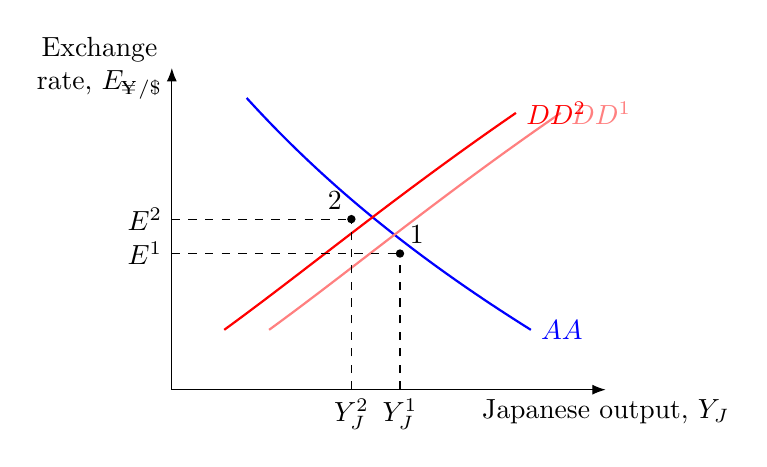
\begin{tikzpicture}[scale=0.95,>=Latex]
\draw[->] (0,0) -- (0,4.3) node[left,align=center]{Exchange\\rate, $E_{\text{¥}/\$}$};
\draw[->] (0,0) -- (5.8,0) node[below]{Japanese output, $Y_J$};

\draw[thick,blue] (1.0,3.9) .. controls (2.0,2.8) and (3.2,1.8) .. (4.8,0.8)
node[right] {$AA$};

\draw[thick,red!50] (1.3,0.8) .. controls (2.4,1.6) and (3.6,2.6) .. (5.2,3.7)
node[right] {$DD^1$};

\draw[thick,red] (0.7,0.8) .. controls (1.8,1.6) and (3.0,2.6) .. (4.6,3.7)
node[right] {$DD^2$};

\fill (3.05,1.82) circle (1.6pt) node[above right] {$1$};
\fill (2.40,2.28) circle (1.6pt) node[above left] {$2$};

\draw[dashed] (3.05,0)--(3.05,1.82);
\draw[dashed] (0,1.82)--(3.05,1.82);
\draw[dashed] (2.40,0)--(2.40,2.28);
\draw[dashed] (0,2.28)--(2.40,2.28);

\node[left] at (0,1.82) {$E^1$};
\node[left] at (0,2.28) {$E^2$};
\node[below] at (3.05,0) {$Y_J^1$};
\node[below] at (2.40,0) {$Y_J^2$};
\end{tikzpicture}
\end{center}

\[
DD:\ \text{left},
\qquad
AA:\ \text{no shift},
\qquad
Y_J \downarrow,
\qquad
E_{\text{¥}/\$}\uparrow.
\]

So Japanese output falls and the yen depreciates.

%-------------------- c --------------------
\item \textbf{An exogenous increase in Japanese real money demand}

An increase in real money demand raises Japanese interest rates at any given level of output:
\[
L(R,Y_J)\uparrow \Rightarrow R_J \uparrow.
\]
Higher Japanese interest rates raise the return on yen deposits, so the yen appreciates:
\[
E_{\text{¥}/\$}\downarrow.
\]
Therefore, the AA curve shifts down.  
The DD curve does not shift.

\begin{center}
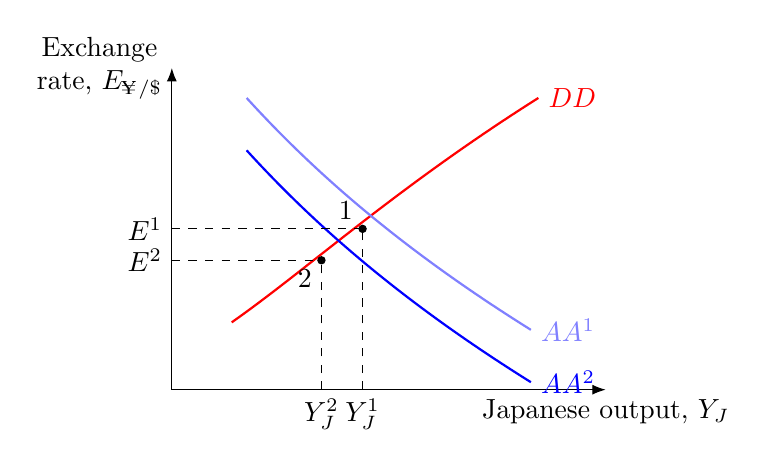
\begin{tikzpicture}[scale=0.95,>=Latex]
\draw[->] (0,0) -- (0,4.3) node[left,align=center]{Exchange\\rate, $E_{\text{¥}/\$}$};
\draw[->] (0,0) -- (5.8,0) node[below]{Japanese output, $Y_J$};

\draw[thick,red] (0.8,0.9) .. controls (1.8,1.6) and (3.0,2.7) .. (4.9,3.9)
node[right] {$DD$};

\draw[thick,blue!50] (1.0,3.9) .. controls (2.0,2.8) and (3.2,1.8) .. (4.8,0.8)
node[right] {$AA^1$};

\draw[thick,blue] (1.0,3.2) .. controls (2.0,2.1) and (3.2,1.1) .. (4.8,0.1)
node[right] {$AA^2$};

\fill (2.55,2.15) circle (1.6pt) node[above left] {$1$};
\fill (2.00,1.73) circle (1.6pt) node[below left] {$2$};

\draw[dashed] (2.55,0) -- (2.55,2.15);
\draw[dashed] (0,2.15) -- (2.55,2.15);
\draw[dashed] (2.00,0) -- (2.00,1.73);
\draw[dashed] (0,1.73) -- (2.00,1.73);

\node[left] at (0,2.15) {$E^1$};
\node[left] at (0,1.73) {$E^2$};
\node[below] at (2.55,0) {$Y_J^1$};
\node[below] at (2.00,0) {$Y_J^2$};
\end{tikzpicture}
\end{center}

\[
DD:\ \text{no shift},
\qquad
AA:\ \text{down},
\qquad
Y_J \downarrow,
\qquad
E_{\text{¥}/\$}\downarrow.
\]

So Japanese output falls and the yen appreciates.

%-------------------- d --------------------
\item \textbf{An increase in U.S. interest rates}

If U.S. interest rates rise, dollar deposits become more attractive relative to yen deposits. To maintain interest rate parity, the dollar must appreciate now and the yen must depreciate now:
\[
R_{\$}\uparrow \Rightarrow E_{\text{¥}/\$}\uparrow.
\]
Therefore, the AA curve shifts up.  
The DD curve does not shift.

\begin{center}
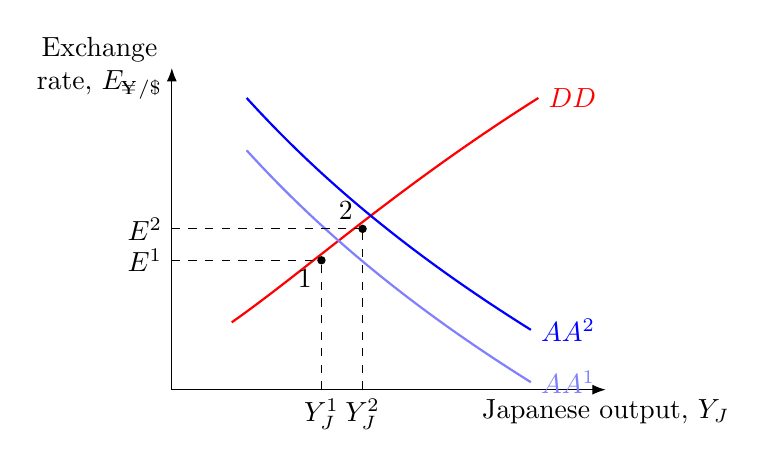
\begin{tikzpicture}[scale=0.95,>=Latex]
\draw[->] (0,0) -- (0,4.3) node[left,align=center]{Exchange\\rate, $E_{\text{¥}/\$}$};
\draw[->] (0,0) -- (5.8,0) node[below]{Japanese output, $Y_J$};

\draw[thick,red] (0.8,0.9) .. controls (1.8,1.6) and (3.0,2.7) .. (4.9,3.9)
node[right] {$DD$};

\draw[thick,blue!50] (1.0,3.2) .. controls (2.0,2.1) and (3.2,1.1) .. (4.8,0.1)
node[right] {$AA^1$};

\draw[thick,blue] (1.0,3.9) .. controls (2.0,2.8) and (3.2,1.8) .. (4.8,0.8)
node[right] {$AA^2$};

\fill (2.00,1.73) circle (1.6pt) node[below left] {$1$};
\fill (2.55,2.15) circle (1.6pt) node[above left] {$2$};

\draw[dashed] (2.00,0) -- (2.00,1.73);
\draw[dashed] (0,1.73) -- (2.00,1.73);
\draw[dashed] (2.55,0) -- (2.55,2.15);
\draw[dashed] (0,2.15) -- (2.55,2.15);

\node[left] at (0,1.73) {$E^1$};
\node[left] at (0,2.15) {$E^2$};
\node[below] at (2.00,0) {$Y_J^1$};
\node[below] at (2.55,0) {$Y_J^2$};
\end{tikzpicture}
\end{center}

\[
DD:\ \text{no shift},
\qquad
AA:\ \text{up},
\qquad
Y_J \uparrow,
\qquad
E_{\text{¥}/\$}\uparrow.
\]

So Japanese output rises and the yen depreciates.

%-------------------- e --------------------
\item \textbf{Japanese consumers decide they want to consume less and save more}

There is a fall in consumption:

\[
C \downarrow \Rightarrow D \downarrow.
\]
So the DD curve shifts left.  
The AA curve does not shift directly.

\begin{center}
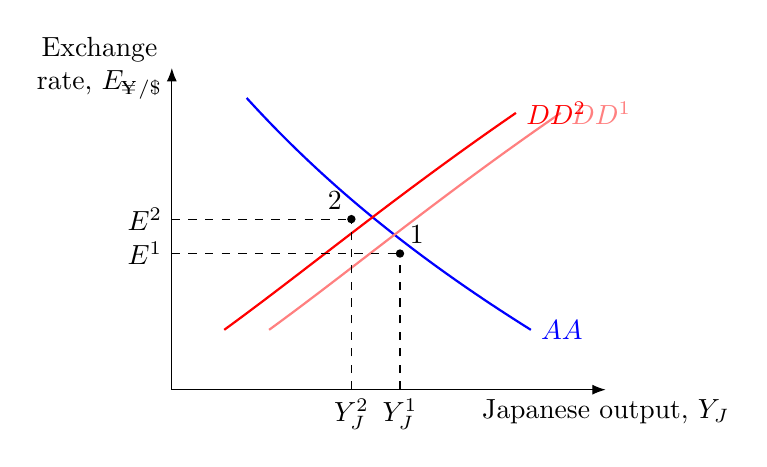
\begin{tikzpicture}[scale=0.95,>=Latex]
\draw[->] (0,0) -- (0,4.3) node[left,align=center]{Exchange\\rate, $E_{\text{¥}/\$}$};
\draw[->] (0,0) -- (5.8,0) node[below]{Japanese output, $Y_J$};

\draw[thick,blue] (1.0,3.9) .. controls (2.0,2.8) and (3.2,1.8) .. (4.8,0.8)
node[right] {$AA$};

\draw[thick,red!50] (1.3,0.8) .. controls (2.4,1.6) and (3.6,2.6) .. (5.2,3.7)
node[right] {$DD^1$};

\draw[thick,red] (0.7,0.8) .. controls (1.8,1.6) and (3.0,2.6) .. (4.6,3.7)
node[right] {$DD^2$};

\fill (3.05,1.82) circle (1.6pt) node[above right] {$1$};
\fill (2.40,2.28) circle (1.6pt) node[above left] {$2$};

\draw[dashed] (3.05,0)--(3.05,1.82);
\draw[dashed] (0,1.82)--(3.05,1.82);
\draw[dashed] (2.40,0)--(2.40,2.28);
\draw[dashed] (0,2.28)--(2.40,2.28);

\node[left] at (0,1.82) {$E^1$};
\node[left] at (0,2.28) {$E^2$};
\node[below] at (3.05,0) {$Y_J^1$};
\node[below] at (2.40,0) {$Y_J^2$};
\end{tikzpicture}
\end{center}

\[
DD:\ \text{left},
\qquad
AA:\ \text{no shift},
\qquad
Y_J \downarrow,
\qquad
E_{\text{¥}/\$}\uparrow.
\]

So Japanese output falls and the yen depreciates.

\medskip
\noindent
\end{enumerate}

\end{problem}

\end{document}